% =====================================================================
%  Matched-Magnitude Controls for Causal Testing of Spectral Mechanisms
%  in Attention.  A short methodological note.
%  Standalone; same toolchain as the Gap-Statement paper.
% =====================================================================
\documentclass[11pt]{article}

\usepackage[utf8]{inputenc}
\usepackage[T1]{fontenc}
\usepackage{amsmath,amssymb}
\usepackage{graphicx}
\usepackage{booktabs}
\usepackage[margin=1in]{geometry}
\usepackage[colorlinks=true,linkcolor=blue,citecolor=blue,urlcolor=blue]{hyperref}

\graphicspath{{figures/}{./}}

\title{\textbf{Matched-Magnitude Controls for Causal Testing of\\
  Spectral Mechanisms in Attention}}
\author{Evgeny Vyaltsev\thanks{ORCID: \texttt{0009-0004-3712-6798}} \and
        Daniil Vyaltsev}
\date{\today}

\begin{document}
\maketitle

% =====================================================================
\begin{abstract}
Mechanistic claims about the spectral structure of attention --- that some
eigenmode, gap, or spectral direction \emph{carries computation} --- are
increasingly common, but they are rarely subjected to a causal test, and
when they are, the test often lacks a control for the magnitude of the
intervention. We argue that this omission is not a detail: an ablation
that suppresses a ``dominant'' spectral mode almost always perturbs the
model by a larger amount than a naive control, and that magnitude
asymmetry alone produces a downstream effect that is easily mistaken for
evidence of a computational mechanism. We give a worked example from our
own work in which a natural intervention construction produced a
treatment perturbation $10$--$30\times$ larger than its control --- an
asymmetry that would have read as a strong positive result --- and was
caught only by a matched-magnitude sanity check before the full run. We
then describe a simple framework --- matched-magnitude intervention, a
random-spectrum baseline, and pre-registered outcome criteria --- and
report that, once the magnitudes were matched, the same hypothesis
returned a pre-registered null. The note is intended as a short, reusable
checklist for anyone running causal tests of spectral mechanisms.
\end{abstract}

% =====================================================================
\section{The problem}
\label{sec:problem}

A recurring pattern in the interpretability of attention is the spectral
mechanistic claim: an eigenvalue, a spectral gap, a dominant eigenvector,
or a low-rank direction of some attention-derived operator is identified,
shown to correlate with model behaviour, and then described as a mechanism
--- something the model \emph{uses} to compute. The spectral object is
real and measurable; the inferential step from ``measurable and
correlated'' to ``computationally load-bearing'' is where the difficulty
lies.

Correlational evidence cannot settle that step. A spectral quantity can be
perfectly reproducible, mathematically well-defined, and tightly coupled
to other quantities, and still be causally inert --- a description of the
computation rather than a part of it. Deep learning offers many such
structures: embedding anisotropy, neuron clusters, loss-landscape valleys.
Each is real; none is, on its own, a mechanism. Distinguishing the two
requires intervention: change the spectral object and measure whether the
computation changes.

Intervention, however, introduces its own failure mode, and it is this
failure mode that the present note is about. An intervention is only
informative relative to a control, and the control must be matched in the
right variable. The variable that matters is the \emph{magnitude of the
perturbation applied to the model}. If the treatment --- ablating the
spectral object of interest --- perturbs the model more than the control,
then any downstream difference is confounded: it may reflect the special
role of the object, or it may reflect nothing more than ``a larger
perturbation does more damage.'' These two explanations are not
distinguishable after the fact. They must be separated by construction,
before the experiment is run.

This is easy to state and easy to violate, because the natural
constructions of a spectral intervention do not preserve perturbation
magnitude. We show this concretely next.

% =====================================================================
\section{A worked example}
\label{sec:example}

We take the example from our own work, because we have the full record of
what went wrong and how it was caught.

\paragraph{The hypothesis.}
The free-energy Hessian of an attention head can be written
$H=-\beta\operatorname{Cov}_p(k)$, where $k$ are the key vectors, $p$ are
the softmax attention weights of a query, and $\beta$ is the
scaled-dot-product temperature. On trained models this Hessian is
typically spike-dominated: one eigenvalue $\lambda_1$ is much larger in
magnitude than the rest. The hypothesis under test was that this dominant
mode is a privileged computational object --- that the model relies on it,
and that removing it should selectively damage next-token prediction.

\paragraph{The intervention.}
To test this causally, one ablates the dominant mode and measures the
downstream effect. The mode is a direction $v_1$ in key space; ablating it
means suppressing the variance of the keys along $v_1$. The control,
correspondingly, suppresses a random non-dominant direction $v_j$ from the
bulk of the spectrum. If the dominant mode is special, the treatment must
hurt \emph{more} than the control.

\paragraph{The naive construction and its hidden asymmetry.}
The first, natural construction was: project the key matrix to remove its
component along the chosen direction, then rescale the result to preserve
the Frobenius norm $\|K\|_F$. Preserving $\|K\|_F$ feels like the right
invariant --- the keys keep their overall scale --- and it is a quantity
one naturally thinks to hold fixed.

It is the wrong invariant. Preserving $\|K\|_F$ does not preserve the
magnitude of the \emph{perturbation} $\|\delta K\|_F$, and the
perturbation magnitude is what the control must match. Removing the
dominant direction $v_1$ deletes a large component of the keys; removing a
bulk direction $v_j$ deletes a tiny one. Rescaling to a common $\|K\|_F$
afterwards does not undo this --- it leaves the treatment having moved the
keys much farther than the control. In our runs the dominant-mode
projection produced a perturbation $\|\delta K\|_F$ that was $10$ to
$30\times$ larger than the bulk-mode control, depending on the
layer--head pair. Concretely, for one early-layer head the dominant
direction carried a key-projection magnitude $M_T\approx 84.9$ against the
bulk direction's $M_C\approx 15.8$ --- a factor of $5.4$ in magnitude, and
larger once expressed as a perturbation norm.

\paragraph{Why this would have looked like a discovery.}
An uncontrolled smoke run with this construction showed the treatment
producing a downstream KL divergence roughly $18\times$ that of the
control. Taken at face value, that is a striking positive result: ``the
dominant spectral mode is far more important than a random mode.'' It is
exactly the number one would hope to see if the hypothesis were true. It
is also entirely consistent with the dominant mode being computationally
irrelevant --- because the treatment had simply perturbed the model
$10$--$30\times$ harder. The experiment, as constructed, could not tell
the two apart. The asymmetry was caught not by inspecting the result ---
the result looked good --- but by a separate sanity check that measured
$\|\delta K\|_F$ for treatment and control directly, before committing to
the full run.

% =====================================================================
\section{Why the naive control deceives}
\label{sec:why}

The mechanism of the deception is worth stating precisely, because it
generalises beyond this one construction.

Any intervention on a model induces a downstream change, and to first
order the size of that change grows with the size of the intervention.
Write the downstream effect as $E(\delta)$, a function of the perturbation
$\delta$ applied. For small perturbations $E$ is monotone increasing in
$\|\delta\|$: a larger push produces a larger effect, almost regardless of
\emph{where} the push is applied. A causal test of ``does direction $A$
matter more than direction $B$'' must therefore compare $E$ at
\emph{equal} $\|\delta\|$. If instead the test compares
$E(\delta_A)$ against $E(\delta_B)$ with $\|\delta_A\|\gg\|\delta_B\|$,
the outcome $E(\delta_A)>E(\delta_B)$ is overdetermined --- it follows from
the magnitude gap alone and carries no information about $A$ versus $B$.

The trap is that the magnitude gap is invisible unless explicitly
measured. The experimenter chooses an invariant to preserve --- here,
$\|K\|_F$ --- believes the comparison is therefore fair, and never inspects
$\|\delta K\|_F$. The preserved invariant and the invariant that actually
needs preserving are different quantities, and nothing in the construction
signals the difference. The result then looks like a clean positive,
because the confound and the hypothesis predict the same sign.

This is a general hazard for spectral interventions specifically, because
spectral objects are defined by magnitude: the ``dominant'' mode is, by
definition, the direction along which the operator has the largest action.
Ablating it is intrinsically a larger intervention than ablating a bulk
mode. The asymmetry is not a bug in one construction; it is built into
what ``dominant'' means. Any spectral causal test that does not
explicitly neutralise it will tend to confirm the mechanism whether or not
the mechanism is real.

% =====================================================================
\section{The framework}
\label{sec:framework}

The remedy is not elaborate. It has three components, and the value of
stating them as a checklist is precisely that they are easy to omit.

\paragraph{1. Matched-magnitude intervention.}
Construct treatment and control so that the perturbation norm
$\|\delta\|$ applied to the model is equal --- not an indirect invariant
such as the operator norm of the keys, but the perturbation itself. In
our corrected construction this was done by computing, for each
layer--head pair, the key-projection magnitude of both the dominant
direction ($M_T$) and the random bulk direction ($M_C$), and scaling both
interventions to the smaller of the two, $T=\min(M_T,M_C)$. The treatment
and control then move the model by the same amount by construction. After
the fix, the verified treatment-to-control magnitude ratio was $1.000$ on
every layer--head pair tested. Matching the perturbation has a price ---
in our case, exact preservation of $\|K\|_F$ had to be given up, and the
resulting change in $\|K\|_F$ was logged (sub-percent for typical
interventions). That trade is correct: the perturbation match is the
invariant the causal claim depends on; $\|K\|_F$ is not.

\paragraph{2. A random-spectrum baseline.}
Matching magnitude controls for ``how hard did we push.'' A second control
addresses ``is the structure we are testing even non-trivial.'' Before
attributing significance to a spectral object, check whether a random
spectrum --- random eigenvalues of the same dimension, carrying no trained
structure --- exhibits the same property. If it does, the property is a
feature of the spectral summary, not of the trained model. We found this
necessary in practice: a coupling among three spectral summary statistics
that looked like a low-dimensional structure of trained heads turned out
to be reproduced exactly by random spectra --- it was an algebraic
identity among monotone functions of spectral peakedness, not a property
of the network. A random-spectrum baseline catches this class of
non-finding before it is built upon.

\paragraph{3. Pre-registered outcome criteria.}
Fix, before running, what the two outcomes are and what each means. A
causal test is only honest if a null result is as reportable as a
positive one. We pre-registered: if the matched treatment-minus-control
effect was statistically indistinguishable from zero, the dominant-mode
hypothesis was to be declared null and the direction closed; if the
treatment effect significantly exceeded the control, the hypothesis would
continue. Writing this down in advance removes the post-hoc freedom to
reinterpret a null as ``a weak positive'' or to explain it away.

% =====================================================================
\section{Result of applying the framework}
\label{sec:result}

With the three components in place, the hypothesis of
Section~\ref{sec:example} was tested on Llama-3.2-1B over WikiText-2:
twelve layer--head pairs spanning early, middle, and late layers, each on
twenty-five prompts, $300$ measurements in total, at a context length of
$256$ keys. Each measurement compared three forward passes --- unablated
baseline, dominant-mode treatment, matched bulk-mode control --- on the
same prompt.

\begin{table}[t]
  \centering
  \caption{Matched-control ablation of the dominant spectral mode. The
  operationally meaningful metric --- next-token NLL --- shows a
  treatment-minus-control differential whose $95\%$ confidence interval
  brackets zero. The result is a pre-registered null.}
  \label{tab:result}
  \begin{tabular}{lrrrr}
    \toprule
    Metric & $\overline{\Delta}_{\mathrm{treat}}$
           & $\overline{\Delta}_{\mathrm{ctrl}}$
           & differential & Wilcoxon $p$ \\
    \midrule
    NLL (next-token) & $5.95\times10^{-4}$ & $3.23\times10^{-4}$
      & $+2.72\times10^{-4}$ & $0.26$ \\
    KL (distribution) & $1.31\times10^{-3}$ & $7.81\times10^{-4}$
      & $+5.32\times10^{-4}$ & $<10^{-38}$ \\
    \bottomrule
  \end{tabular}
\end{table}

The outcome is shown in Table~\ref{tab:result}. On next-token NLL --- the
operationally meaningful measure --- the treatment-minus-control
differential is $+2.7\times10^{-4}$, with a $95\%$ confidence interval of
$[-1.7\times10^{-4},\,7.0\times10^{-4}]$ that brackets zero, and a
Wilcoxon signed-rank $p=0.26$. By the pre-registered criterion this is a
null: suppressing the dominant spectral mode harms next-token prediction
no more than suppressing a random bulk mode of the same perturbation
magnitude. As a fraction of the baseline NLL the differential is
$\sim10^{-4}$ --- operationally negligible, independently of the
significance test. The effect did not concentrate in any layer band; the
per-band differentials are individually consistent with zero.

The KL divergence between treatment and control output distributions is
statistically distinguishable from zero ($p<10^{-38}$), but its absolute
scale is $\sim5\times10^{-4}$ nats, and it does not translate into NLL
harm. A detectable distributional shift that does not affect task
performance is consistent with the dominant mode being a description of
the computation rather than a load-bearing part of it.

The contrast with the uncontrolled smoke run is the point of this note.
The same hypothesis, with the same model and the same kind of
intervention, returned a treatment KL of roughly $18\times$ the control
under the naive construction and a null under the matched construction.
The difference between a reported discovery and a reported null was
entirely the magnitude match. Figure~\ref{fig:matched} shows the
verification that, after the fix, the treatment and control perturbation
magnitudes were equal across all twelve pairs.

\begin{figure}[t]
  \centering
  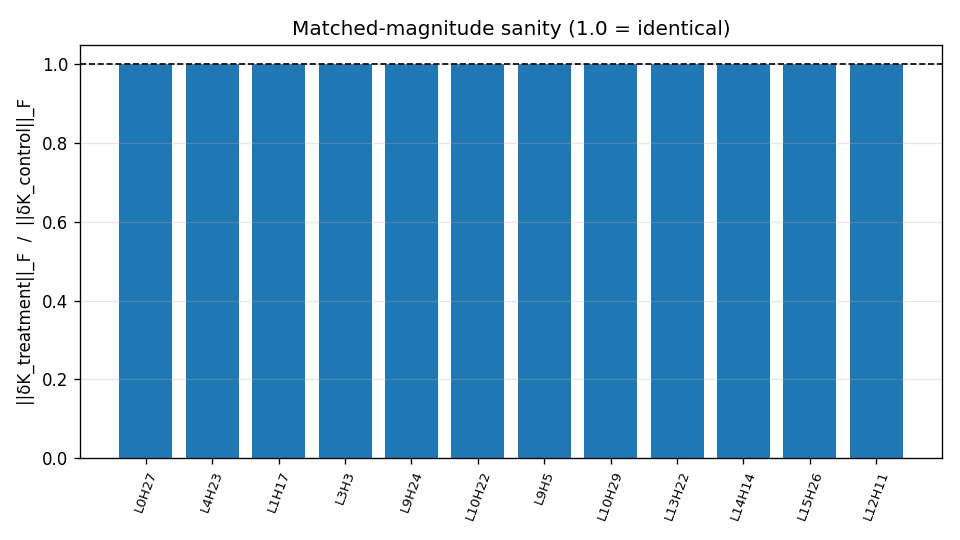
\includegraphics[width=0.78\textwidth]{matched_magnitude.png}
  \caption{Matched-magnitude verification. For each of the twelve
  layer--head pairs, the perturbation magnitude applied in the treatment
  (dominant-mode ablation) and in the control (random bulk-mode ablation)
  after the corrected construction. The ratio is $1.000$ across all pairs:
  the two interventions move the model by the same amount, so the
  downstream comparison is not confounded by perturbation size. Under the
  naive $\|K\|_F$-preserving construction this ratio was $10$--$30$.}
  \label{fig:matched}
\end{figure}

% =====================================================================
\section{Recommendation}
\label{sec:recommendation}

We close with the checklist the note argues for. It is short by design;
its usefulness is that each item is easy to skip and costly to skip.

\begin{enumerate}
  \item \textbf{Match the perturbation, not a proxy.} Construct treatment
    and control so that the perturbation norm $\|\delta\|$ applied to the
    model is equal. Do not substitute an indirect invariant (operator
    norm, parameter norm) for the perturbation itself --- they are
    different quantities, and only the perturbation match neutralises the
    magnitude confound.
  \item \textbf{Measure the match; do not assume it.} Compute and report
    $\|\delta_{\mathrm{treat}}\|/\|\delta_{\mathrm{ctrl}}\|$ explicitly. A
    construction that looks symmetric can carry a large hidden asymmetry;
    the only way to know is to measure it, before the full run.
  \item \textbf{Add a random-structure baseline.} Check whether a random
    spectrum of the same dimension reproduces the property under study. If
    it does, the property is algebraic, not a fact about the trained
    model.
  \item \textbf{Pre-register both outcomes.} State, before running, what
    constitutes a null and what constitutes a positive, and commit to
    reporting a null as such. A spectral causal test is only evidence if
    it could have come out the other way.
  \item \textbf{Separate the distributional from the operational.} A
    significant KL shift is not a mechanism if it does not move the
    task-level metric. Report both, and do not let a small significant
    distributional effect stand in for an operational one.
\end{enumerate}

\noindent
None of this is specific to attention or to the particular Hessian we
studied; it applies to any causal test of a spectral object in a trained
network. The reason to write it down is empirical: we adopted exactly one
of these five items late, by accident of a sanity check, and it converted
what would have been a reported positive into a correct null. The other
four are cheap insurance against the same class of error.

\paragraph{Data and code.}
The intervention construction, the matched-magnitude verification, and the
full ablation results are available with the spectral-gap-statement
research record at \url{https://doi.org/10.5281/zenodo.20257482}.

\end{document}
